%%%%%%%%%%%%%%%%%%%%%%%%%%%%%%%%%%%%%%%%%%%%%%%%%%%%%%%%%%%%%%%
%
% Introduction.tex (part of thesis.tex)
% author: Qie Hu
%
%%%%%%%%%%%%%%%%%%%%%%%%%%%%%%%%%%%%%%%%%%%%%%%%%%%%%%%%%%%%%%%

%!TEX root = ../../thesis.tex

\section{Model Identification}\label{sec:model_id}

\subsection{Building Model}
The data-driven model identified for the fourth floor of SDH in Chapter \ref{chapter:building_model} is used here in our field experiments.
To recap, we model the room temperature evolution as follows:
\begin{equation}
\begin{aligned}\label{eq:building_model}
x_{k+1} &= A x_k + B u_k + C v_k + q_k, \\
\end{aligned}
\end{equation}
where $x \in \mathbb{R}^6$ represents the average temperature in each of the six zones on the fourth floor (see Figure \ref{fig:floor_plan}), $u \in \mathbb{R}^6$ is the input vector that contains the total airflow to each zone, $v:= \left[ v_\text{Ta}, v_\text{Ts} \right]^\top \in \mathbb{R}^2$ is a disturbance vector that describes ambient air temperature and the HVAC system's SAT and  $q \in \mathbb{R}^6$ represents the internal gains due to occupancy and electric devices.
Finally, $A$, $B \in \mathbb{R}^{6\times6}$ and $C \in \mathbb{R}^{6\times2}$ are coefficient matrices.


%%%%%%%%%%%%%%%%%%%%%%%%%%%%%%%%%%%%%%%%%%%%%%
%%%%%%%%%%%%%%%%%%%%%%%%%%%%%%%%%%%%%%%%%%%%%%
%%%%%%%%%%%%%%%%%%%%%%%%%%%%%%%%%%%%%%%%%%%%%%
%%%%%%%%%%%%%%%%%%%%%%%%%%%%%%%%%%%%%%%%%%%%%%


\subsection{Fan Model}

A fan model is identified from 6 weeks of one-minute resolution data for the supply fans collected from sMAP.
The fan laws state that the airflow rate through the fan is proportional to the fan speed, and the fan power is a cubic function of its speed \cite{Hvac_book}. 
Figure \ref{fig:fan_model} confirms the linear relationship between the airflow rate and the fan speed. 
The same figure also shows that there is little difference between the best fit quadratic and cubic curves for the relationship between the fan power and fan speed, suggesting that for the range of fan speeds plotted, a quadratic function can describe this relationship without significant loss of accuracy compared to a cubic function. %for fan speed between 28\% and 90\% of its maximum.
%The best fit quadratic and cubic curves for the relationship between the fan power and fan speed are also shown in the figure and they suggest that a quadratic function is able to describe this relationship without significant loss of accuracy compared to a cubic function. 
Since a quadratic function would simplify the subsequent controller design problem, it is adopted in this work. 
%Assume both supply fans are controlled to the same speed. 
%Let $N$ denote the fan speed of both fans, $u$ the total airflow rate through the fans and $P$ the total power consumption of the fans, then the fan model is defined as follows:
Let $N$ denote the fans' speed, $u$ the total airflow through the fans and $P$ the total fan power consumption, then the fan model is given as follows:
\begin{equation}\label{eq:fan_model}
\begin{aligned}
N & = f(u) = a_1 u + a_2\\
P & = g(N) = b_1 N^2 + b_2 N + b_3\\
P & = h(u) = c_1 u^2 + c_2 u + c_3.\\
\end{aligned}
\end{equation} 

\begin{figure}[h]
\centering
\vspace*{1cm}
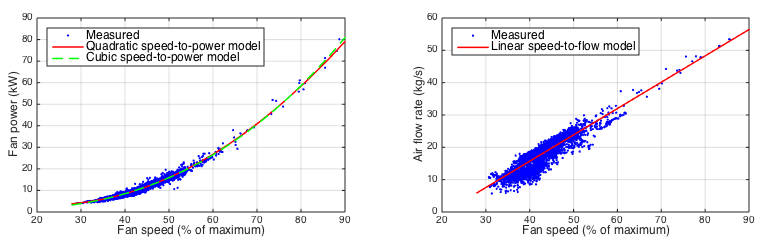
\includegraphics[width=\textwidth]{chapters/building_exp/figures/fan_model.png}
\caption{Fan measurements and identified models for fan power and air flow as functions of fan speed.}
\label{fig:fan_model}
\vspace*{-0.15cm}
\end{figure}








